\section{Overview of Blockchain Naming Systems}

\begin{table}
	\begin{tabular}{r l l}
		\toprule
		Name system & TLDs & Proxies \\
		\midrule
		Namecoin & .bit & BDNS \\
		Emercoin & .lib, & PeerName,  \\
		& .bazar, & friGate, \\
		& .coin, & OpenNIC \\
		& .emc & \\
		Handshake & \emph{any string} & hns.to, \\
		& & NextDNS, \\
		& & HDNS.io,\\
		& & BobWallet extension, \\
		& & LinkFrame extension \\
		ENS & .eth & eth.link, \\
		& & eth.limo \\
		Unstoppable & .crypto, & Brave browser, \\
		& .blockchain, & Opera browser, \\
		& .bitcoin, & Unstoppable browser, \\
		& .coin, & Unstoppable extension, \\
		& .nft, & Infura\\
		& .wallet, & \\
		& .888, & \\
		& .dao, & \\
		& .x, & \\
		& .zil & \\
		\bottomrule
	\end{tabular}
	\caption{Non-exhaustive selection of proxies, browsers, 
		and extensions 
		that can be used to access blockchain-based naming 
		systems. \randall{maybe should have a citation for each 
			of these}}
	\label{tab:proxies_and_tlds}
\end{table}

In this section we present an overview of the largest blockchain-based naming 
systems, to provide background on how such systems work in detail. We select 
these systems based on their apparent popularity, as well as 
prior reports and literature that indicate some of them have already been 
abused by malware. These naming systems fall into two categories: systems built 
on naming-specific blockchains, such as Namecoin and Emercoin, whose purpose is 
primarily to store names and records, and systems built on general-purpose 
blockchains, such as Ethereum, that are designed for purposes beyond naming 
systems. These systems also fall into two ``generations:'' Namecoin and 
Emercoin have existed since ~2012 \randall{find the actual times}, while 
Handshake, the Ethereum Name Service (ENS), and Unstoppable Domains are more 
recent inventions. 

All of the blockchain-based naming systems we study differentiate their names 
from DNS domains by inventing alternate top level domains (alt-TLDs). A 
summary of the alt-TLDs used by each naming system is presented in 
Table~\ref{tab:proxies_and_tlds}. Handshake names are slightly different, since 
the goal of the Handshake project is to replace the DNS root zone and make any 
TLD available for purchase --- see Section~\ref{sec:handshake} for more details.

Although each of these systems are blockchain-based naming 
systems, they differ in several key ways, which are relevant to how defenders 
must treat them when they are abused by malware authors. We now summarize each 
system in more detail.

\subsection{Naming-Specific Blockchains}

We study three naming systems that are built on naming-specific blockchains: 
Namecoin, Emercoin, and Handshake. Each naming system is built on its eponymous 
blockchain. 

\subsubsection{Namecoin and Emercoin}

Namecoin and Emercoin are the oldest blockchain-based naming systems. Both were 
intended as additions to traditional DNS: users registered domains that 
resolved to IP addresses using records very similar to DNS records. 
Unfortunately, Namecoin and Emercoin have been subject to a large amount of 
abuse. Kalodner et al. found that only 28 of the 120,000 domains registered in 
Namecoin in 2015 had meaningful web content~\cite{kalodner_namecoin_2015}. 
Casino et al. collected all of the IP addresses that names in Emercoin and 
Namecoin resolved to, and submitted them to threat intelligence services 
including VirusTotal, Hybrid Analysis, Abuse.ch, and Pydnsbl (an aggregator of 
blocklists). They found that over 50\% of the IPs in Namecoin and Emercoin 
records had been flagged as malicious by at least one threat intelligence 
service~\cite{casino_unearthing_2021}. Furthermore, Casino et al. used a 
``poisoning'' approach to find IP addresses associated with malicious IPs, 
either because they were stored in the same wallet, the name resolved to them, 
or the same email was recorded in their records. This ``poisoning'' approach 
revealed that the vast majority of IP addresses in Namecoin and Emercoin 
records are 
connected in some way to malicious IPs~\cite{casino_unearthing_2021}.


\subsubsection{Handshake}
\label{sec:handshake}
\begin{table}
	\begin{tabular}{lr}
		\toprule
		Record & Names with Record \\
		\midrule
		Default NS and GLUE4 records & 102,386 \\
		\hspace*{0.2in} No A records & 102,285\\
		\hspace*{0.2in} A 44.235.163.135 & 94 \\
		\hspace*{0.2in} A 52.43.158.89 & 4 \\
		\hspace*{0.2in} A 144.91.114.245 & 2 \\
		\hspace*{0.2in} A 1.1.1.1 & 1 \\
		Invalid name & 98,068 \\
		No record (null) & 845 \\
		TXT record & 138 \\
		\hspace*{0.2in} ``hello fx-wallet'' & 110 \\
		\hspace*{0.2in} Other & 28 \\
		Non-default NS record & 32 \\
		Non-default GLUE4 record & 11 \\
		Distributed storage address & 7 \\
		\midrule
		Total unique names & 201,458 \\
		Total records & 201,487 \\
		\bottomrule
	\end{tabular}
	\caption{Record types in the Handshake namespace.}
	\label{tab:handshake_records}
\end{table}

Handshake is a new blockchain-based system that aims to 
replace the root DNS 
zone. As such, it offers its users the ability to purchase 
nearly any string to 
use as a TLD. Rather than selling second-level domains 
itself, the Handshake ecosystem purports to allow its users 
to act as registrars who can sell their own domains. 
Handshake records are designed to store the NS records of traditional 
authoritative nameservers, rather than to replace DNS A, AAAA, or similar 
records. However, we note that nothing 
restricts malware authors from recording the IP addresses of C2 servers as NS 
records, or running an authoritative nameserver and a C2 server on the same 
machine. Handshake also allows users to store TXT records, which can 
contain the addresses for decentralized web hosting systems 
like Skynet or IPFS. Malware users could potentially use 
Handshake as a naming system to find content stored in 
content-addressed distributed storage systems. Additionally, Handshake 
advertises themselves as ``the only naming blockchain with a lightweight 
recursive DNS resolver, which you can easily embed into 
browsers, apps, and devices''~\cite{namebase_access_handshake}. 
This lightweight resolver may be attractive to malware authors because it is 
small enough to use as part of a malware payload.

\randall{Summarize the .music debate and cite it somewhere.}

We collected a sample of approximately 201,000 recent Handshake names by 
scraping a Handshake block explorer.\footnote{https://e.hnsfans.com/names} We 
attempted to scrape these names 
directly from the Handshake blockchain, but were unsuccessful because the RPC 
provided by the Handshake client to interact with the Handshake node is no 
longer functional: so many names are recorded in the system that the RPC cannot 
return them to the user anymore~\cite{hns_rpc_too_big}. 
Table~\ref{tab:handshake_records} 
summarizes our findings. At the moment, Handshake names appear to be 
overwhelmingly used as speculative assets. Only 0.14\% of names in our sample 
had records that led to either IP addresses or DS addresses, assuming the 
non-default nameserver and glue records do lead to IP addresses or DS 
addresses. Nearly half of registered Handshake domains in our sample cannot be 
resolved by the HNS client, since they contain illegal characters like emojis 
or are solely composed of numbers: these names are nevertheless allowed to be 
minted.

\randall{Because these names seem to have very few records and we can't look 
them all 
up, we don't pay Handshake much attention from here on out.}

\subsection{Naming Systems on General Purpose Blockchains}

A new generation of naming systems based on the Ethereum blockchain have 
recently arrived on the scene. The Ethereum Name Service (ENS) was the first 
\randall{maybe}, followed by Unstoppable Domains. These naming systems are 
possible because of Ethereum's innovation in the blockchain space: \emph{smart 
contracts.} Smart contracts are, in essence, code that is embedded into the 
Ethereum blockchain. Any full node that runs Ethereum can execute any smart 
contract. Each contract is identified by a hexadecimal address, and makes its 
functions available through its ABI. Thus, asking a smart contract to execute 
its function is similar to making an RPC call, except that the user does not 
know or care which physical machine actually executes the code. 

While smart contracts' functionality has some limitations, they can 
be used to implement key-value stores, which means they can act as naming 
systems. For example, in a simplified system, a user might wish to set the name 
``foo.crypto'' to resolve to the IP address 1.2.3.4. The user would create an 
Ethereum transaction that asks the smart contract that 
controls the key-value store to set a record for ``foo.crypto'' to ``1.2.3.4.'' 
This transaction is then broadcast to the Ethereum network, and every Ethereum 
node that receives it updates its own copy of the key-value store to include 
the new record. Reading from the key-value store works similarly to writing to 
it: any Ethereum node can return a correct response. %Implication: taking down 
%the host of a name on Ethereum is not possible without taking down every 
%Ethereum node. In contrast to IPFS, where only one machine stores the content 
%you're looking for, so taking it down might be a lot easier.

Interestingly, systems like ENS and Unstoppable Domains are structured like 
DNS, but they are not necessarily being used as DNS replacements. Both ENS and 
Unstoppable Domains use certain smart contracts as registries, and ENS even 
uses other contracts as resolvers and registrars. However, users are primarily 
using these systems to map human-readable names to \emph{wallet addresses} 
instead. While users can still store IP addresses or traditional domains, very 
few choose to do so.  
%Implication: malware users that store IP addresses, domains, or websites stand 
%out.

Some users store the addresses for distributed 	storage systems, but the 
majority of configured records store wallet addresses. We also 
note that a high percentage of names on ENS and Unstoppable Domains are not 
configured to have records at all. There may be a few reasons why: first, names 
resolve to the wallet address that owns them by default \randall{true on 
	Unstoppable?}, which may be the only use some customers require. Second, 
	while 
purchasing a domain is very straightforward and only requires using a website, 
adding a record requires interacting with smart contracts on the blockchain, 
because only the owner of the domain may modify its records. The company that 
sold the domain no longer has the ability to add records for the user unless 
the user chooses to park their domain in the company's wallet-hosting service. 
This requirement is not obvious at the purchasing step. Third, a large number 
of names appear to be purchased as speculative assets rather than because users 
wish to utilize them directly. 

We now describe the workings of two Ethereum-based naming systems: the 
Ethereum Name Service (ENS) and Unstoppable Domains. 
\subsubsection{ENS}

\begin{table}
	\begin{tabular}{lrr}
		\toprule
		Resolver Name & Txns Setting Resolver & Address \\
		\midrule 
		Public Resolver 2 & 33,304 & \texttt{0x4976fb...} \\
		Public Resolver 1 & 2,736 & \texttt{0xDaaF96...} \\
		OpenSea ENS resolver & 482 & \texttt{0x9C4e9C...} \\
		ENS Old Public Resolver 2 & 440	& \texttt{0x226159...} \\
		Umbra: Stealth Resolver & 409 & \texttt{0xB37671...} \\
		\textit{unnamed PublicResolver} & 126 & \texttt{0xD3ddcC...} \\
		\textit{unnamed PublicResolver} & 103 & \texttt{0x5FfC01...} \\
		ENS Old Public Resolver 1 & 29 & \texttt{0x1da022...} \\
		\bottomrule
	\end{tabular}
	\label{tab:ens_resolvers}
	\caption{The ENS resolvers from which we collected a sample of names and 
		records.}
\end{table}

\begin{figure}[t]
	\centering
	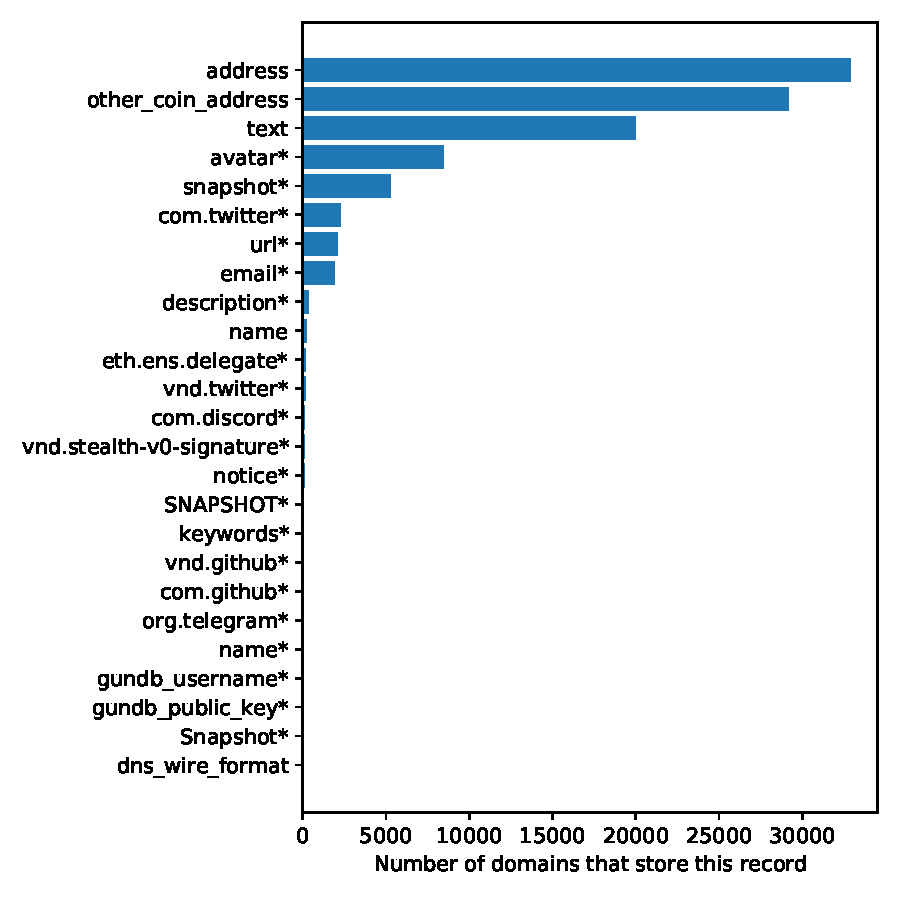
\includegraphics[width=3in]{figs/ens_names.pdf}
	\caption{Records stored by ENS names. *key within ``text'' record}
	\label{fig:ens_records}
\end{figure}

ENS names use smart contracts to fill the roles of the single registrar and 
multiple resolvers in the system. When claiming a name for the first 
time, the user sends a transaction from their wallet to the ENS Registrar 
Controller 
contract, requesting that the name be registered and transferred to the 
ownership of the wallet. The ENS Registrar Controller sets a number of default 
values, including a default wallet 
address record that maps the name to the wallet address that owns it, and a 
default resolver contract for the 
name, which at the moment is the ``ENS Public Resolver 2'' smart 
contract.\footnote{The public 
	resolver contract was updated in the past, and almost all ENS names have 
	now 
	changed their resolvers away
	from the ``Old'' resolvers, usually to the current default resolvers.} To 
	fully 
resolve a 
name, a user must first query the ENS Registrar Controller to determine the 
name's designated resolver, and then query that resolver for the record 
associated with the name. Resolver contracts are allowed to access the storage 
of the ENS Registrar Controller, which means they don't have to perform another 
transaction for the resolver to know that a new record has been created by the 
ENS Registrar Controller. 

Users cannot query a resolver for a name's records directly: they must first 
convert the name to its keccak256 hash. These 
name hashes are referred to as ``nodes.'' Because keccak256 hashes are not 
reversible, 
translating a node back to a name is a non-trivial process. Some name owners 
choose to register their node-to-name mapping in the ``ENS Reverse Registrar'' 
contract, but this practice is not required. While it is possible to enumerate 
all of the transactions that recorded new names from the Registrar Controller 
Contract (and its historical predecessors, such as a contract that was used to 
register short names earlier in ENS's lifetime), this approach still yields some
nodes for which names were never recorded. 

requires another contract, the ENS Reverse 
Registrar. Names are not required to have entries in the ENS Reverse Registrar, 
so this contract is not always able to translate a given node 
back to a name. 

One more notable feature of ENS names is that anyone may renew 
them, not just their owners. The reason for this design choice 
is unclear.

To study this ecosystem, we took a sample of names from the eight resolver 
contracts that were set by the most names as their default resolver. We chose 
eight because the distribution of resolvers is long-tailed: the majority of 
resolvers resolve only a few names, while the eight most popular resolvers 
resolve the majority of names. We excluded addresses that were set as resolvers 
by many names but did not implement the ENS resolver specification, under the 
assumption that these were mistakes. Such misconfigured resolver addresses 
include the null address, 
0x0, as well as other smart contracts used by the ENS ecosystem, such as the 
``Base Registrar Implementation.''  The remainder of the resolvers we chose are 
detailed in Table~\ref{tab:ens_resolvers}.

At the time that we performed this study, 667,369 ENS names had been 
registered through the Registrar Controller contract. Names that did not 
specify a resolver when they were registered 
were assigned the default ENS Public Resolver 2, which presumably accounts for 
the vast majority of the names that never performed an explicit transaction 
setting their resolver. \randall{I'm in the middle of checking this.} 

Figure~\ref{fig:ens_records} shows the distribution of the types of records 
stored by our sample of names. The majority resolve to wallet addresses or text 
records, not IP addresses, traditional domains, or DS addresses. We broke down 
the text records, which are key/value pairs, by the most common key names: 
these keys are marked with an asterisk. Only the most common 25 keys are shown. 
We note that only 17 names had \texttt{dns\_wire\_format} records, which are 
intended to store traditional DNS 
records, and all 17 are malformed as far as we can tell. \randall{should maybe 
	work on that some more? Couldn't tell what was wrong by examining the 
	octets.}

%Describe the registrar/registry/resolver structure. We took a sample 
%of X domains from the most 
%frequently updated resolver contracts.
%
%Haven't found anything bad yet except loli-hentai.x. This 
%system, like all other uncensorable systems, will probably 
%eventually attract CSAM. Describe what we did to find 
%domains, how I crawled a subset.

\subsubsection{Unstoppable Domains}

\begin{figure}[t]
	\centering
	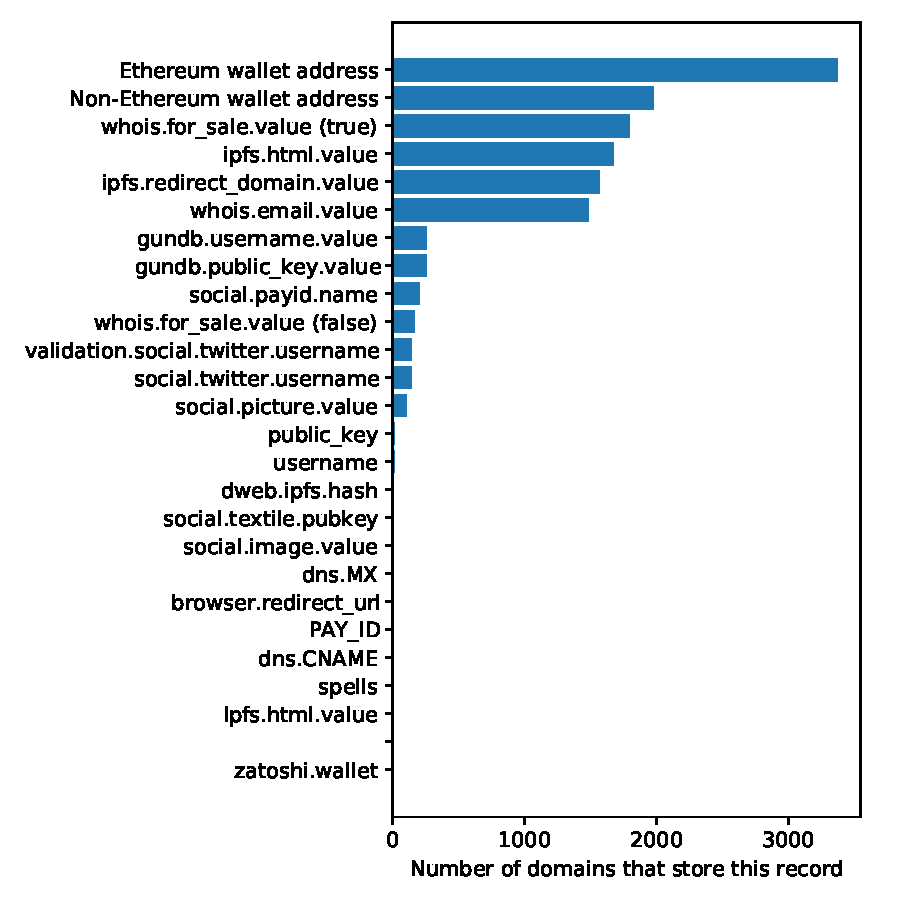
\includegraphics[width=3in]{figs/all_unstoppable_records.pdf}
	\caption{Records stored by Unstoppable Domains names.}
	\label{fig:unstoppable_records}
\end{figure}

%Describe the registry contract and the crawled domains (I did 
%crawl these didn't I?)

Like ENS, Unstoppable Domains uses Ethereum smart contracts as 
registrars. Unstoppable names are divided into two systems. CNS 
(Crypto Name System) contains all names with \texttt{.crypto} 
TLDs, and has separate registry and resolver contracts. This 
system was created first. Later, Unstoppable added UNS 
(Unstoppable Name System), which simplified name resolution by 
combining the resolver and registry contracts, and added several 
new TLDs. Unstoppable names never have to be renewed; they are 
purchased once and then owned for life. This is primarily 
because Unstoppable Domains does not have the capability to 
reclaim a name unless the private key of the owning wallet is 
known to them. 

Unstoppable names are referenced by their namehashes, which are 
similar to ENS's ``nodes.'' We extracted all namehashes from the 
Unstoppable Domains registry contract by searching all of its 
transactions, and then found each name's records by querying 
Unstoppable's metadata endpoint.\footnote{
	\texttt{https://metadata.unstoppabledomains.com/metadata/}} 
Figure~\ref{fig:unstoppable_records} shows the 
distribution 
of record types found in the Unstoppable Domains names. As in 
ENS, the majority of names have wallet records rather than 
records that point to websites in any way. The next most common 
type of record is ``whois.for\_sale.value,'' showing that many 
names are seen as speculative assets. Unstoppable Domains also 
provides an easy way for users to link to IPFS records. IPFS, 
the ``Inter-Planetary File System,'' is a distributed 
blockchain-based hosting service that allows users to host 
static websites.

We performed a web crawl of all of the Unstoppable names that 
had records pointing to websites, whether IPFS records, 
traditional IP addresses, or traditional domains. We took 
screenshots of the 367 websites we arrived 
at, inspected them manually, and did not find any evidence of 
malware use. Most 
websites were personal sites, Web3-based business sites, or related to the sale 
or collection of NFTs. 

We also examined the sample of names from B-root for any Unstoppable Domains 
names that appeared to be associated with malware. 

Unstoppable Domains has claimed that their naming system is not well suited for 
malware authors or other miscreants for two reasons. First, Unstoppable Domains 
claims to police which domains may be sold. The CEO of Unstoppable Domains, 
Matthew Gould, stated in an email that Unstoppable ``prevented the 
registration of domains associated with known pirating software or other types 
of IP theft and fraud''~\cite{pegoraro_blockchain_2021}. Second, Unstoppable 
can also seize a domain if that 
domain is hosted by Unstoppable's custody 
wallet, instead of by a private wallet~\cite{pegoraro_blockchain_2021}. In 
fact, other wallet hosting 
services, such as Coinbase's, 
could presumably also seize wallets that store domains, since the private 
keys of those wallets are 
known to the service. However, we note that seizing hosted wallets may not 
be a reliable 
intervention, because malware authors can evade this tactic by simply using 
self-hosted wallets. 

